\section{Data}
To answer the challenge I needed the following data points:
\medskip
\begin{enumerate}
  \item Number of inhabitants per province in the Netherlands
  \item Average house price per province in the Netherlands
  \item Number of restaurants per province in the Netherlands
\end{enumerate}
\medskip
Ad 1. The number of inhabitants per province in the Netherlands can be downloaded from the Centraal Bureau voor Statistiek \textbf{(CBS)}: a government owned, freely accessible web site with tons of statistical datasets (over 4K of them!) to use in all kind of analysis. I did some research on which table would best provide my need for the number of inhabitants per province and its title turns out to be \texttt{[Regionale kerncijfers Nederland]}. The resulting data frame, including some data cleaning done like removing substring \texttt{[(PV)]} from the province name, is in figure \ref{inhabitant}.  
\\\\
Ad 2. The average house price per province in the Netherlands in 2019 also can be downloaded from the CBS, this time based on the table with title \texttt{[Bestaande koopwoningen; gemiddelde verkoopprijzen, regio]}. After a bit of cleaning and tweaking (i.e. 'Friesland' ≠ 'Fryslân' and some column renaming had to be adjusted to make the dataset comprehensible for our international readers) the resulting data frame is in figure \ref{avgprice}.
\\\\
Ad 3. The third dataset, the number of restaurants, came from FourSquare. I needed to find all restaurants within each province of the Netherlands. The FourSquare API has the following two drawbacks that I needed to overcome: the non commercial API limits the returned number of venues per call to max 100 and although the results have a \texttt{[state]} field, the API doesn't allow searching per state. The limit of max 100 venues per call I overcame with the help of the material I found of a fellow course student Guillermo (G.) Bareirro \cite{STUDENT1}. FourSquare returns max 100 venues per call, but if you make the call specific enough, the total results will not grow above the limit. Using the categories listed bij G. Bareirro, I was able to split querying all restaurants into their separate categories and thereafter grouped and summed them with pandas standard data frame functionality. To overcome the second drawback of not being able to query FourSquare by state and knowing that an estimate of the restaurants per province would be sufficient for my analyses, I queried the restaurants (via their respective subcategories) in the capital city of each province. For the province of Noord-Holland I made an exception: the capital of Noord-Holland is Haarlem, but Amsterdam (the capital of the Netherlands) is by far a more important city in the province of Noord-Holland so I took the liberty of using Amsterdam instead of Haarlem as the anchor point for the FourSquare queries. The data frame is in figure \ref{restaurants}.
\\\\
The three data frames used in the analyses for this assignment are in the images below:
\medskip
\begin{figure}[H]
	\begin{subfigure}{0.33\textwidth}
		\centering
		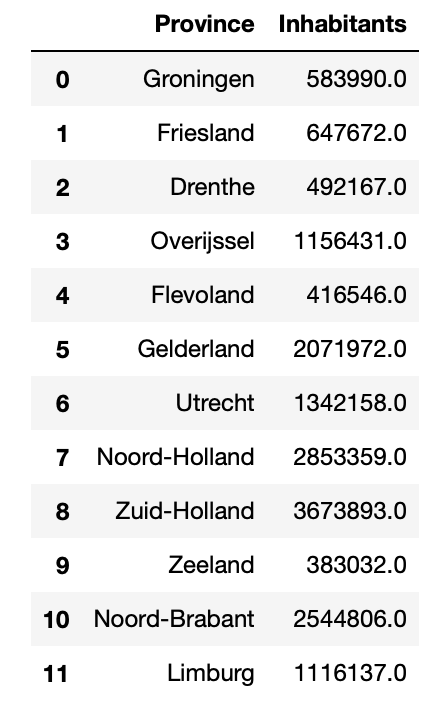
\includegraphics[scale=.4]{Inhabitants.png} 
		\caption{Inhabitants from StatLine \cite{CBS1}}
		\label{inhabitant}
	\end{subfigure}
	\begin{subfigure}{0.33\textwidth} 
		\centering 
		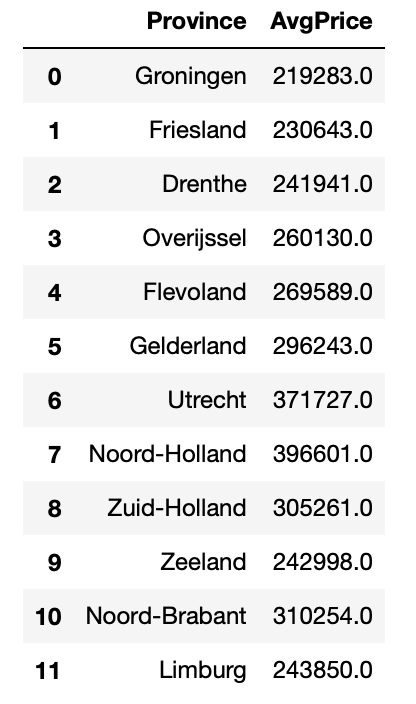
\includegraphics[scale=.4]{AvgPrice.png} 
		\caption{Average Price from StatLine \cite{CBS2}}
		\label{avgprice}
	\end{subfigure}
	\begin{subfigure}{0.33\textwidth}
		\centering
		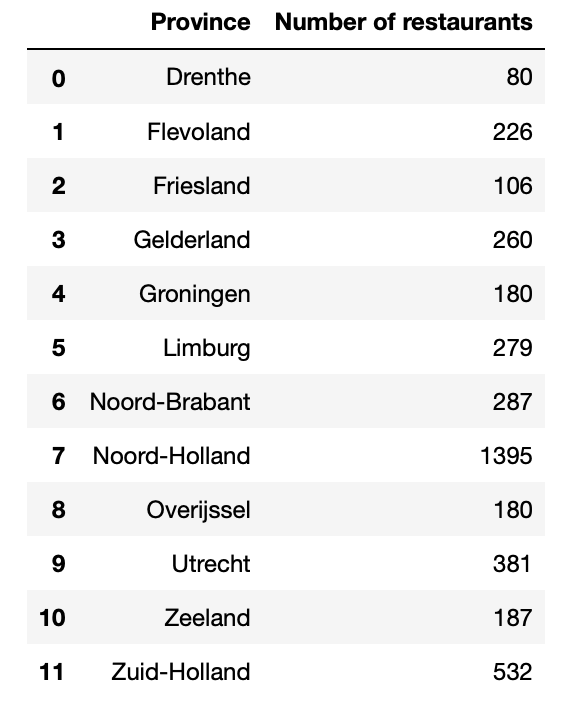
\includegraphics[scale=.4]{Restaurants.png} 
		\caption{Restaurants from FourSquare \cite{FS2}}
		\label{restaurants}
	\end{subfigure}
\caption{Cleaned data frames as used in analysis}
\end{figure}
\medskip
After submitting this data section for the first part of my graduation I came across a dataset that turned out to be very helpful in showing the final results on a map of the Netherlands and it was too compelling for me to leave this opportunity out of this report. So the fourth part added to the data frames was a \textbf{GeoPandas} data frame with the geometries of each province in the Netherlands. Thanks to the excellent blog post of Artem (A.) Zapara \cite{STUDENT2} I was able to get the final bit of information I needed and added it to the resulting data frame of figure \ref{resultset}.
\medskip
\begin{figure}[H]
	\center
	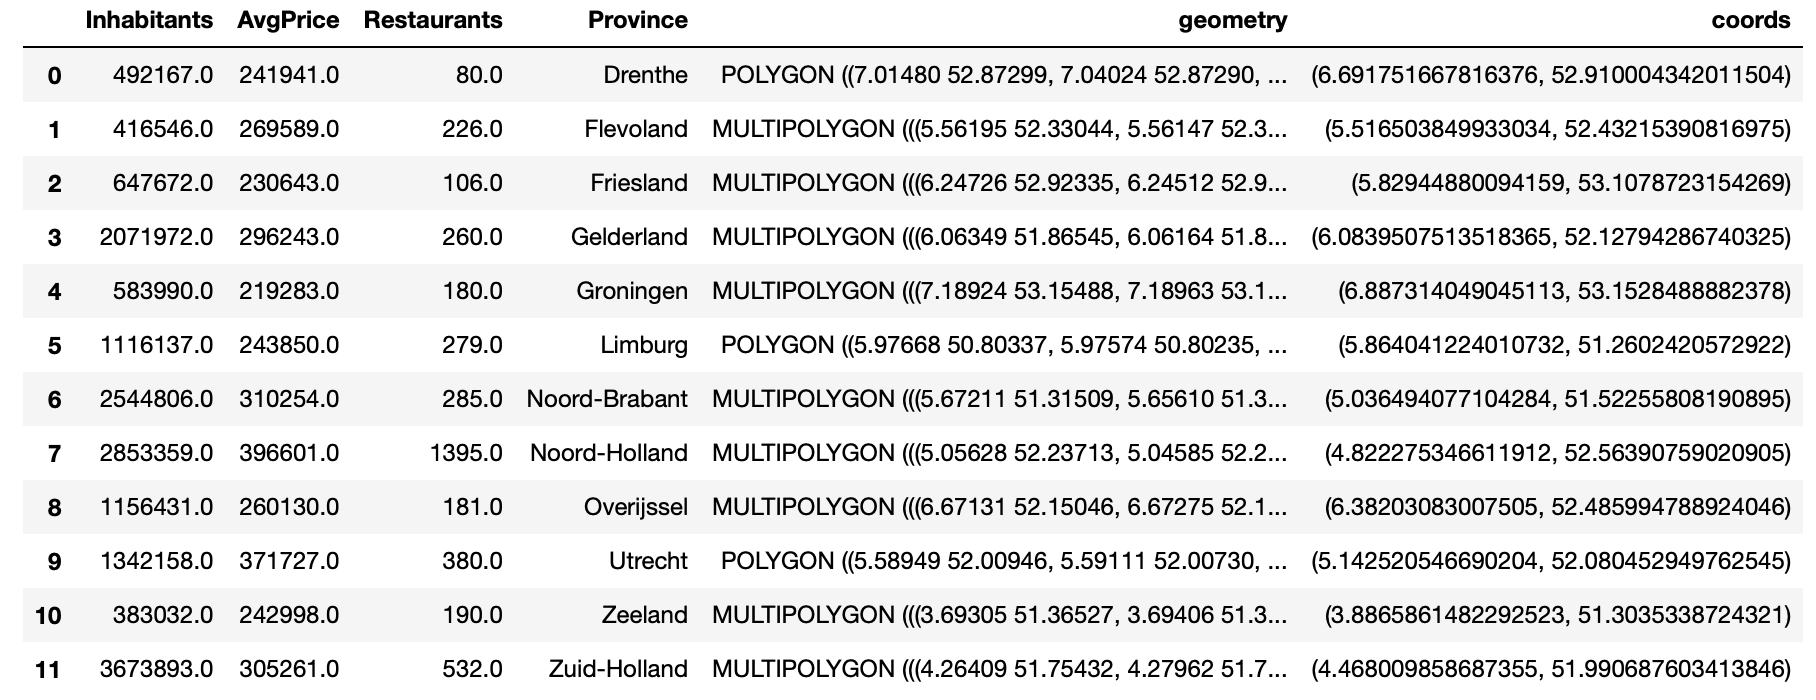
\includegraphics[scale=.4]{ResultSet.png}	
	\caption{Result set for analyses and reporting}
	\label{resultset}
\end{figure}
\medskip
As always I was very impressed with the work of fellow programmers / students: almost any programming question already has been answered (although sometimes in parts) and can be found on Google. If you know the right keywords and have enough time to keep searching, you will find most of the puzzle pieces readably available. You just need to connect the dots so to say. On top of that, Python keeps amazing me for the strength of its coding syntax: import the right libraries and with just a couple of lines of code you can generate, filter and merge data frames into a data frame ready for takeoff.


